\documentclass[conference,letterpaper]{IEEEtran}
% ISCAS 2027 specifies IEEEtran conference mode. Do not shrink class fonts or margins.
\usepackage[T1]{fontenc}
\usepackage{newtxtext,newtxmath}
\usepackage{amsmath}
\usepackage{booktabs,array,tabularx}
\usepackage{graphicx}
\usepackage{tikz}
\usetikzlibrary{arrows.meta,positioning,calc}
\usepackage{cite}
\usepackage[hidelinks]{hyperref}
\usepackage{microtype}
\hypersetup{pdftitle={EP-L2: Elastic Payload Storage for In-Place Writeback in GPU L2 Caches},pdfauthor={EP-L2 project -- author details pending},pdfsubject={English working manuscript; no accepted application results}}
\newcommand{\epl}{EP-L2}
\newcommand{\base}{B16}
\newcommand{\unif}{U-WB16}
\newcommand{\pending}{\textemdash}
\newcommand{\workingnote}{\noindent\fbox{\parbox{\dimexpr\columnwidth-2\fboxsep-2\fboxrule\relax}{\footnotesize\textbf{Working manuscript.} Application measurements and physical implementation results remain pending. Dashes denote unavailable results, not zero effects.}}}
\newcolumntype{L}[1]{>{\raggedright\arraybackslash}p{#1}}
\hyphenation{write-back micro-ar-chi-tec-ture in-di-rec-tion}
\begin{document}
\title{EP-L2: Elastic Payload Storage for\ In-Place Writeback in GPU L2 Caches}
\author{\IEEEauthorblockN{Author information to be completed}
\IEEEauthorblockA{English working draft EN-v1 --- not for submission}}
\maketitle

\begin{abstract}
A dirty line can lose its resident tag before its data have been accepted by the lower memory system, while its writeback-ordering state may remain live even longer. In the fixed-partition L2 reference studied here, moving a dirty line from resident storage to a writeback buffer consumes bank service, while idle capacity in another partition cannot be borrowed. We propose Elastic Payload L2 (EP-L2), which separates tag visibility, physical data ownership, and writeback ordering. A dirty victim becomes writeback-staged in its original payload slot; the incoming resident line receives a different, bank-compatible slot. Against a fixed-partition reference, the design retains the same payload capacity and bank-service budget, removes the resident-to-writeback copy, and permits cross-role allocation. We specify the ownership and release protocol, derive storage and control costs, and define matched experiments that distinguish fewer bank operations, relief of capacity pressure, and application performance. Independently qualified application results and physical implementation measurements are pending; this draft reports no empirical speedup or area benefit.
\end{abstract}
\begin{IEEEkeywords}
GPU, L2 cache, writeback buffer, tag--data decoupling, resource sharing
\end{IEEEkeywords}

\section{Introduction}
A shared GPU L2 serves resident hits, outstanding misses, and dirty evictions using resources with different lifetimes. A resident tag provides address lookup; a payload slot holds data; miss metadata tracks requests and returns. During a dirty eviction, an address-ordering entry may also remain allocated after the local writeback data have been transferred. Treating these resources as one object can retain a resource after its own responsibility has ended.

This paper studies an L2 organization with separate quotas for resident, bypass-return, and writeback-buffer (WBUF) data. The reference copies a dirty resident line into WBUF before reusing its resident slot. That copy consumes a source-bank read and a destination-bank write; sending the staged line downstream requires a further bank read. Increasing WBUF capacity can relieve a capacity limit, but does not remove this transfer. Conversely, eliminating the transfer need not help a workload that is limited elsewhere.

Our observation is that \emph{a change in the consumer of a data line need not require a change in its physical location}. \epl{} replaces the fixed role-to-location relationship with explicit payload ownership. On a dirty eviction, the old payload remains in place for writeback, while a different slot is assigned to the incoming resident line. The resident-tag budget is unchanged: additional nonresident slots do not create additional resident lookup entries.

Tag--data indirection itself is established practice, for example in V-Way caches~\cite{vway}. The focus here is its use across \emph{resident and transient data lifetimes}, with the associated storage, bank operations, and release events accounted for explicitly. Our contribution is an in-place writeback protocol under a fixed payload budget, together with a bank-matched reference and an evaluation design that separates copy elimination from capacity sharing. Optional victim-retention and read-only paths use the same ownership framework, but are not prerequisites for evaluating writeback pooling.

The central question is therefore not whether a unified allocator can be implemented, but whether it improves useful L2 service under actual pressure, and whether that improvement reaches application execution time. We keep capacity, transport, and throughput claims separate throughout the design and evaluation.

\section{Architecture and Ownership Protocol}
\subsection{Reference Organization and Data Budget}
Table~\ref{tab:configuration} fixes the primary comparison. Each slice has 1024 resident tags and 1168 line-sized payload slots. The reference, \base{} (\texttt{B16\_BANKED}), partitions these slots into 1024 resident, 128 bypass, and 16 WBUF entries. \unif{} (\texttt{U\_WB16}) shares the same slots across roles. Both organizations have four banks, each providing at most one line-sized operation per \emph{physical} GPU cycle. A common 128-byte copy latch is outside the allocatable pool in both designs. Equal data capacity and bank service do not imply equal control cost, area, energy, or clock frequency.

\begin{table}[t]
\caption{Primary configuration. Capacities are per slice unless stated.}
\label{tab:configuration}
\centering\footnotesize
\begin{tabularx}{\columnwidth}{@{}L{0.40\columnwidth}X@{}}
\toprule
Resource & Configuration \\
\midrule
Resident tags & 64 sets $\times$ 16 ways = 1024 \\
Line / sectors & 128 B / four 32-B sectors \\
Payload data, \base{} / \unif{} & 1168 slots = 146 KiB in either mode \\
Payload banks & 4 $\times$ 292 slots; 1 operation/bank/cycle \\
Common copy latch & 128 B; not allocatable as a payload \\
Request descriptors & 512, shared by all applicable paths \\
Line-MSHRs / requesters & 128 entries / at most 32 per address \\
Writeback address directory & 128 entries \\
L2-to-DRAM queue & 128 entries \\
Chip organization & 64 slices; 32 memory channels \\
DRAM / scheduler / return & 850 MHz; 128 / 192 entries per channel \\
L1 & Fixed 64 KiB/core; 4 banks; 20-cycle setting \\
\bottomrule
\end{tabularx}
\end{table}

A payload handle contains a slot identifier and generation number. Tags and transient transactions refer to a handle rather than assuming that tag index equals payload index. Each slot has one authoritative owner, with sector-ready, sector-pending, and pin state protecting outstanding users. The initial design preserves the resident bank class:
\begin{equation}
\operatorname{bank}(p)=p\bmod 4=\operatorname{tag\_index}\bmod 4.
\label{eq:bankclass}
\end{equation}
This restriction prevents a change in resident bank placement from being conflated with pooling. It also means that a nonempty global free pool does not guarantee a legal landing slot for a particular replacement.

\subsection{Dirty Eviction Without a Resident-to-WBUF Copy}
Figure~\ref{fig:paths} contrasts the two paths. Before changing a dirty victim, the controller reserves the address-ordering entry, required issue resources, and a legal data destination. In \base{}, it reads the resident bank, writes WBUF through the copy latch, and later reads WBUF to send the data downstream. Bank conflicts serialize operations under the same service limit as demand traffic.

In \unif{}, the dirty victim's payload changes role to \texttt{WB\_STAGED} without changing location. The controller assigns a distinct bank-compatible slot to the incoming resident line and updates its tag-to-payload association. The writeback still pays for the lower-send bank read and downstream queue occupancy. Pooling therefore removes the copy, not the need to transport writeback data or to reserve its receiving storage.

\begin{figure}[t]
\centering
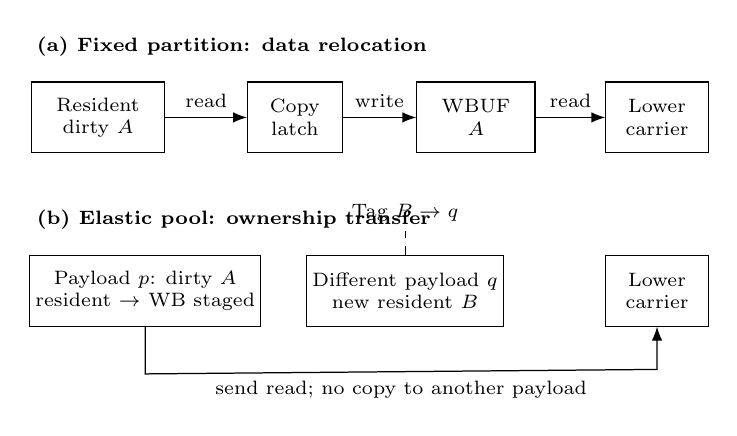
\begin{tikzpicture}[x=1mm,y=1mm,>=Latex,font=\scriptsize,
 box/.style={draw,minimum height=9mm,align=center,inner sep=2pt},
 arr/.style={->,line width=.45pt}]
\node[anchor=west,font=\scriptsize\bfseries] at (0,33) {(a) Fixed partition: data relocation};
\node[box,minimum width=17mm] (br) at (9,24) {Resident\\dirty $A$};
\node[box,minimum width=12mm] (bl) at (34,24) {Copy\\latch};
\node[box,minimum width=15mm] (bw) at (57,24) {WBUF\\$A$};
\node[box,minimum width=13mm] (bd) at (80,24) {Lower\\carrier};
\draw[arr] (br)--node[above]{read} (bl);
\draw[arr] (bl)--node[above]{write} (bw);
\draw[arr] (bw)--node[above]{read} (bd);
\node[anchor=west,font=\scriptsize\bfseries] at (0,11) {(b) Elastic pool: ownership transfer};
\node[box,minimum width=28mm] (up) at (15,2) {Payload $p$: dirty $A$\\resident $\to$ WB staged};
\node[box,minimum width=24mm] (uq) at (48,2) {Different payload $q$\\new resident $B$};
\node[box,minimum width=13mm] (ud) at (80,2) {Lower\\carrier};
\draw[arr] (up.south)--++(0,-6)--node[below]{send read; no copy to another payload} (80,-8)--(ud.south);
\draw[dashed] (uq.north)--++(0,3) node[above] {Tag $B\to q$};
\end{tikzpicture}
\caption{Writeback data movement, not a cycle-accurate schedule. Both modes use the same payload capacity and bank budget. The copy latch remains provisioned in both. The new resident is assigned $q\ne p$ in the elastic path.}
\label{fig:paths}
\end{figure}

Reservations are transactional: a failure leaves the old tag, data, owner, and pending state intact. Once a request is accepted, its return has a reserved landing location. Optional retention must not consume resources needed for mandatory writeback progress. The writeback drain path does not require successful allocation for a new resident request; progress additionally relies on eventual service by the existing bank arbiter and lower memory system. This is a local design requirement, not a proof that arbitrary whole-GPU configurations are deadlock-free.

\subsection{Tag Visibility, Data Ownership, and Address Ordering}
The release events are distinct (Fig.~\ref{fig:lifetimes}). Let $t_r$ denote the committed ownership transfer, $t_a$ the lower system's actual acceptance of the data, and $t_d$ writeback completion. The old tag can be reused after the replacement commits, but the staged payload remains protected until $t_a$. The writeback address directory (WAD) maintains same-address ordering until $t_d$. Reservations may begin before $t_r$.

\begin{figure}[t]
\centering
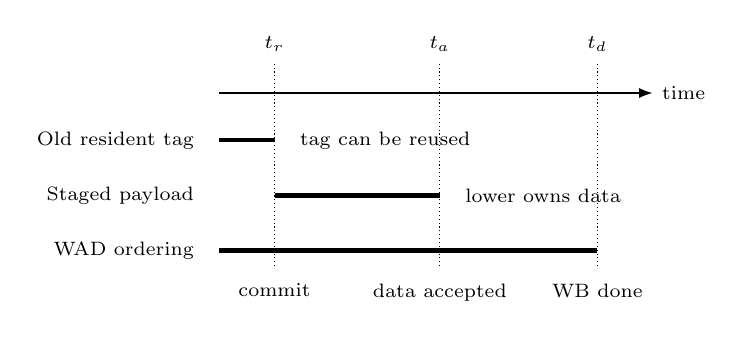
\begin{tikzpicture}[x=1mm,y=1mm,>=Latex,font=\scriptsize]
\draw[->] (31,20)--(86,20) node[right]{time};
\foreach \x/\lab in {38/{$t_r$},59/{$t_a$},79/{$t_d$}} {
 \draw[densely dotted] (\x,-2)--(\x,24);
 \node[above] at (\x,24) {\lab};
}
\node[anchor=east] at (29,14) {Old resident tag};
\node[anchor=east] at (29,7) {Staged payload};
\node[anchor=east] at (29,0) {WAD ordering};
\draw[line width=1.6pt] (31,14)--(38,14);
\draw[line width=1.6pt] (38,7)--(59,7);
\draw[line width=1.6pt] (31,0)--(79,0);
\node[anchor=west] at (40,14) {tag can be reused};
\node[anchor=west] at (61,7) {lower owns data};
\node[below,align=center] at (38,-3) {commit};
\node[below,align=center] at (59,-3) {data accepted};
\node[below,align=center] at (79,-3) {WB done};
\end{tikzpicture}
\caption{Distinct release events in the WB-only design. A WAD entry may remain live after the local writeback data are released. Optional TVD retention creates an additional owned-data lifetime, not a free copy.}
\label{fig:lifetimes}
\end{figure}

For example, dirty line $A$ may retain payload $p$ while its former tag entry names line $B$ at payload $q$. A late event for $A$ must use $A$'s transaction identity and cannot update $B$ through the reused tag index. At $t_a$, the local staging slot may be released only after the lower path has a separately accounted data carrier. A pointer enqueued in a simulator is not, by itself, a physical data transfer. The WAD entry can outlive that slot until the real completion callback.

Correct operation requires three invariants: live and reserved payloads never exceed the physical pool; every completion refers to the appropriate live generation and requested sectors; and payload or descriptor release follows the actual consumer's acceptance, not a speculative enqueue attempt. Pins retain data during bank reads and response backpressure. Partial-sector readiness never implies that an entire line is ready.

\subsection{Optional Consumers of the Same Pool}
A transient victim directory (TVD) retains useful victim data without a resident tag. It shares a 128-entry address-directory budget with WAD, gives mandatory writeback priority, and adds one lookup cycle after a tag miss. Reads use only valid requested sectors. A clean victim must be promoted before a write or atomic operation; dirty in-flight reads may be forwarded, while writes and atomics wait for writeback completion. These retained payloads remain explicitly owned and cannot be reclaimed merely because their staging role has ended.

The read-only (RO) extension independently enables pending-tag detachment and Line-MSHR bypass. A complete-commandlist, line-granular closed-world oracle excludes writes, atomics, and unproven external updates. A detached transaction retains its handle and request state; a late fill completes its original consumers without reinstalling a replaced tag. Both extensions are disabled in the primary \base{}/\unif{} comparison and require separate validation. Neither receives an additional payload array or descriptor pool.

\section{Evaluation Methodology and Result Status}
\subsection{Matched Execution and Functional Validation}
The implementation targets the Accel-Sim/GPGPU-Sim SASS simulation flow~\cite{accelsim}. The primary comparison switches \base{} and \unif{} in the \emph{same repaired binary}, with identical non-mode configuration, complete trace contents, commandlist scope, and termination rules. It is a study of the declared L2 organization, not a claim to reproduce an undocumented commercial GPU cache. The sensitivity comparison uses 8 WBUF entries: both organizations then contain 1160 payload slots, or 145 KiB per slice.

The fixed development set comprises convolutionSeparable, FWT\_7\_21, cfd\_097k, vectorAdd\_4M, and sad. The last is a low-pressure negative control. Btree and dwt2d are reserved for validation after policy choices are fixed; scan is a separate long-running case. All completed matched results, including slowdowns, must be retained. The full-set geometric mean is defined only after all five pairs meet the same acceptance criteria.

Validation exercises the actual cache and partition paths. Nonzero host-memcpy offsets must not reset bank arbitration within a physical GPU cycle; tag-replacement timestamps and timed data service use their respective clocks. Untimed host prefill must establish valid tag--payload associations, preserve unrelated sectors, and reject dirty, pinned, pending, or nonquiescent state before mutation. Directed cases also cover generation reuse, partial and reordered sector returns, response backpressure, writeback acceptance and completion, and final resource drain.

The SASS application traces do not provide complete numerical payloads. Model validation therefore uses independent symbolic sector-version checks and ownership, requester, and transaction identities; it does not establish full numerical application correctness. Instruction-count agreement and normal termination are necessary checks, not substitutes for these invariants. New measurements require independent validation of the actual producing source and binary.

\subsection{Separate Copy, Capacity, and Throughput Effects}
\textbf{Copy cost.} For one otherwise equivalent completed writeback episode in the stated reference, the staging path uses three logical bank operations: source read, destination write, and send read. The in-place path uses the send read only. This is a protocol-level count, not a measured speedup. Application totals must still count actual evictions and bank operations in each run: a different eviction count cannot be normalized away as a presumed fixed saving. Retries are not additional logical operations.

\textbf{Capacity sharing.} A role transition or a nonzero borrowing counter is insufficient evidence. We measure staged-data occupancy and residence time, reserved slots, static WBUF-full waits, pool-full waits, eligible-slot failures, and allocation sources. Capacity benefit requires both binding static partition pressure and useful allocation from otherwise inaccessible capacity. WAD-full stalls are tracked separately because pooling data does not enlarge address-ordering capacity.

\textbf{Application performance.} For equal instruction counts and a common timing scope, the speedup is
\begin{equation}
 S=C_{\base}/C_{\unif}.
\end{equation}
Bank waiting time is a sum over operations, not elapsed GPU cycles that can simply be subtracted from execution time. We therefore relate bank service and admission improvements to lower-queue occupancy, actual lower/DRAM traffic, and complete application cycles. Extra concurrent writebacks can move pressure downstream rather than improve throughput.

\subsection{Conditional Controls and Pending Results}
When measured capacity sharing contributes, an equal-1168-slot static repartition, such as 1024 resident/112 bypass/32 WBUF, tests whether a fixed allocation suffices. Its smaller bypass partition is an explicit cost. When copy savings could explain the difference, a separately qualified equal-copy-service diagnostic is needed to isolate that effect. Neither control adds ports or unaccounted storage.

If L2 service improves but application time does not, a representative case can use a four-point comparison: baseline/mechanism crossed with the original downstream configuration/one justified headroom setting. This separates interaction with the mechanism from the benefit of simply accelerating memory. Optimistic WB-capacity, metadata-capacity, and read-hit diagnostics use their own same-binary baseline and are not realizable \epl{} results.

\begin{table}[t]
\caption{Reserved main-result panel. No qualified application pair is currently available. Each row must use the same accepted binary and matched input.}
\label{tab:pending}
\centering\footnotesize
\begin{tabular}{@{}lccc@{}}
\toprule
Workload & Cycles B/U & Copy ops B/U & Speedup \\
\midrule
convolutionSeparable & \pending & \pending & \pending \\
FWT\_7\_21 & \pending & \pending & \pending \\
cfd\_097k & \pending & \pending & \pending \\
vectorAdd\_4M & \pending & \pending & \pending \\
sad & \pending & \pending & \pending \\
\bottomrule
\end{tabular}
\end{table}

\workingnote
\par\smallskip
No performance number from an earlier, invalidated implementation enters Table~\ref{tab:pending}. The eventual result section must pair its main performance plot with copy operations, true staging pressure, and bank/lower-path service evidence. At present, neither an application benefit nor a negative performance conclusion is established.

\section{Storage Cost and Implementation Requirements}
The primary data budget is $1168\times128$ B $=146$ KiB per slice, plus the common 128-B latch. Across 64 slices, payload storage is 9.125 MiB and latches add 8 KiB. These quantities exclude metadata, ECC, SRAM periphery, and interconnect. The lower data carriers are accounted for separately and identically in both modes.

A slot index requires $P=\lceil\log_2 1168\rceil=11$ bits. Let $A$ be address width, $G$ generation width, and $K$ pin-count width. The implementation's three allocation roles, eight states, line-address key, generation, four ready bits, four pending bits, and pin count give the illustrative independent-field representation
\begin{equation}
 S_{\mathrm{slot}}=N[2+3+(A-7)+G+4+4+K]\ \mathrm{bits}.
\end{equation}
This is a gross encoding model, not incremental area or a proven minimum. Role/state correlation may permit compression, but requires an actual encoding; chosen generation and pin widths require live-reference and wraparound bounds.

\begin{table}[t]
\caption{Selected control-state accounting; omitted fields remain costs, not free resources. $P=11$.}
\label{tab:cost}
\centering\footnotesize
\begin{tabularx}{\columnwidth}{@{}L{.37\columnwidth}X@{}}
\toprule
Component & Accounting requirement \\
\midrule
1024 tag handles & $1024(P+G)$ bits if generation is stored explicitly \\
Up to 128 WB handles & $128(P+G)$ bits, plus state and transaction binding \\
Replacement reservation & $3(P+G)+P+10+2+4$ known bits, plus address, binding, and rollback state \\
Allocation control & Bank-compatible free-slot selection and role/pin checks \\
Bank arbitration & Bounded pending tokens, selection, retry state, and fairness logic \\
Optional directories & Shared WAD/TVD lookup; RO completion state sized from its actual implementation \\
\bottomrule
\end{tabularx}
\end{table}

Some of these fields are already common to the pointerized reference. A final hardware comparison must identify shared, removed, and added state instead of charging all fields only to \epl{}. Symbolic reference versions used by the simulator are verification state, not substitutes for payload RAM or automatically required hardware.

The timing-critical paths are tag-to-handle validation and bank selection, replacement reservation and free-slot selection, and the WB-send read followed by lower acceptance. A software scan or map does not provide zero-cost allocation or lookup. The one-operation bank budget constrains service, but does not establish that the added control meets the same clock. Matched RTL, SRAM macros, synthesis, and timing constraints are not yet available; no area, power, or frequency number is claimed. Energy estimation likewise requires measured event counts and corresponding macro/control energy, without double-counting the eliminated copy accesses.

\section{Related Work and Scope}
V-Way~\cite{vway} separates tag and data placement to support demand-based associativity and global replacement. \epl{} does not claim tag--data indirection as a new idea; it uses explicit ownership to share resident and transient \emph{payload} capacity while retaining a fixed resident-tag budget. Victim caching~\cite{victim} motivates retaining displaced lines for reuse, but the WB-only comparison here does not rely on victim hits. Its optional TVD must be evaluated separately. Adaptive GPU miss handling~\cite{dlmshr} addresses miss-tracking resources; the primary \epl{} experiment holds descriptor and Line-MSHR budgets fixed rather than treating extra metadata as payload-pooling benefit.

\section{Conclusion}
\epl{} separates resident visibility, data ownership, and writeback ordering so that dirty data can remain in place when their consumer changes. The design removes resident-to-WBUF copying under an equal payload and bank-service budget, while exposing idle capacity to other roles. Whether these changes relieve actual capacity pressure and improve application execution remains an empirical question. The matched evaluation and explicit cost model are designed to answer that question without conflating data movement, storage capacity, or additional hardware resources.

\begin{thebibliography}{1}
\bibitem{vway}
M.~K. Qureshi, D.~Thompson, and Y.~N. Patt, ``The {V-Way} cache: Demand-based associativity via global replacement,'' in \emph{Proceedings of the 32nd Annual International Symposium on Computer Architecture (ISCA)}, 2005, pp. 544--555.
\bibitem{accelsim}
M.~Khairy, Z.~Shen, T.~M. Aamodt, and T.~G. Rogers, ``{Accel-Sim}: An extensible simulation framework for validated {GPU} modeling,'' in \emph{Proceedings of the 47th Annual International Symposium on Computer Architecture (ISCA)}, 2020, pp. 473--486.
\bibitem{victim}
N.~P. Jouppi, ``Improving direct-mapped cache performance by the addition of a small fully-associative cache and prefetch buffers,'' in \emph{Proceedings of the 17th Annual International Symposium on Computer Architecture (ISCA)}, 1990, pp. 364--373.
\bibitem{dlmshr}
Y.~Gu and L.~Chen, ``Dynamically linked {MSHRs} for adaptive miss handling in {GPUs},'' in \emph{Proceedings of the International Conference on Supercomputing (ICS)}, 2019, pp. 510--521.
\end{thebibliography}
\end{document}
